\documentclass[a4paper,12pt]{article}
\usepackage[utf8]{inputenc}
\usepackage[italian]{babel}
\usepackage{graphicx}
\usepackage{listings}
\usepackage{xcolor}
\usepackage{float}
\usepackage{hyperref}
\usepackage{geometry}
\usepackage{amsmath}
\usepackage{booktabs}

\geometry{
 a4paper,
 total={170mm,257mm},
 left=20mm,
 top=20mm,
}

\definecolor{codegreen}{rgb}{0,0.6,0}
\definecolor{codegray}{rgb}{0.5,0.5,0.5}
\definecolor{codepurple}{rgb}{0.58,0,0.82}
\definecolor{backcolour}{rgb}{0.95,0.95,0.92}

\lstdefinestyle{mystyle}{
    backgroundcolor=\color{backcolour},   
    commentstyle=\color{codegreen},
    keywordstyle=\color{magenta},
    numberstyle=\tiny\color{codegray},
    stringstyle=\color{codepurple},
    basicstyle=\ttfamily\footnotesize,
    breakatwhitespace=false,         
    breaklines=true,                 
    captionpos=b,                    
    keepspaces=true,                 
    numbers=left,                    
    numbersep=5pt,                  
    showspaces=false,                
    showstringspaces=false,
    showtabs=false,                  
    tabsize=2
}

\lstset{style=mystyle}

\title{\textbf{Relazione Progetto NLP: Classificazione Automatica di Curriculum Vitae}}
\author{Team Data Science}
\date{\today}

\begin{document}

\maketitle

\tableofcontents
\newpage

\begin{abstract}
Questo documento presenta l'implementazione e l'analisi di una pipeline di Natural Language Processing per la classificazione automatica di Curriculum Vitae in 24 categorie professionali. Utilizzando un dataset di 2484 documenti, abbiamo sviluppato un approccio basato su feature TF-IDF e un classificatore Linear SVC. Nonostante le sfide legate allo sbilanciamento delle classi e alla sovrapposizione semantica, il modello raggiunge un'accuratezza di baseline del 52\%. Il report discute criticamente le scelte metodologiche, i limiti dell'attuale preprocessing (es. perdita di keyword tecniche) e propone linee guida per l'adozione di modelli basati su Transformer per iterazioni future.
\end{abstract}

\section{Introduzione}
Il presente report descrive il lavoro svolto per la realizzazione di una pipeline di Machine Learning volta alla classificazione automatica di Curriculum Vitae (Resume). L\'obiettivo principale è stato quello di sviluppare un sistema in grado di assegnare una categoria lavorativa (es. HR, Engineering, Designer) a partire dal contenuto testuale del CV.

Il progetto si basa sul dataset \texttt{Resume.csv}, contenente 2484 curriculum etichettati in 24 categorie diverse.

\section{Analisi e Preprocessing dei Dati}

\subsection{Dataset}
Il dataset di partenza è composto dalle seguenti colonne principali:
\begin{itemize}
    \item \texttt{Resume\_str}: Il contenuto testuale del CV.
    \item \texttt{Category}: La categoria lavorativa di appartenenza (target).
\end{itemize}

Dall'analisi esplorativa è emerso che il dataset presenta un certo grado di **sbilanciamento** tra le classi. Mentre categorie come \textit{INFORMATION-TECHNOLOGY} o \textit{BUSINESS-DEVELOPMENT} contano circa 120 esempi ciascuna, altre come \textit{BPO} o \textit{AUTOMOBILE} sono significativamente meno rappresentate (rispettivamente 22 e 36 esempi). Per mitigare questo problema durante la fase di training, abbiamo adottato una strategia di suddivisione dei dati **stratificata** (vedi Sez. Metodologia), garantendo che la proporzione delle classi fosse mantenuta in tutti i set (Train, Validation, Test).

\subsection{Pulizia del Testo (Text Cleaning)}
Per migliorare la qualità delle feature estratte, abbiamo implementato una fase di preprocessing specifica. In particolare, abbiamo notato che molti CV iniziavano con intestazioni interamente in maiuscolo che potevano introdurre bias nel modello.
La funzione di pulizia implementata esegue i seguenti passaggi:
\begin{enumerate}
    \item Rimozione delle parole iniziali scritte interamente in maiuscolo (spesso indicanti il ruolo, che svelerebbe la label).
    \item Conversione di tutto il testo in minuscolo.
    \item Rimozione della punteggiatura.
    \item Rimozione di spazi bianchi superflui.
\end{enumerate}

\textit{Critica alle scelte di Preprocessing:} In questa implementazione preliminare sono emerse tre debolezze metodologiche significative:
\begin{enumerate}
    \item \textbf{Euristica sui Job Title:} La rimozione delle parole iniziali in maiuscolo (pensata per filtrare intestazioni generiche) è rischiosa. Spesso l'incipit del CV contiene il Job Title esatto (es. "JAVA DEVELOPER"), che è la feature più predittiva. Eliminandolo, si penalizza il modello basandosi sull'errata convinzione che usare il titolo costituisca "Data Leakage", mentre è un dato legittimo.
    \item \textbf{Mancata Normalizzazione:} L'assenza di Lemmatizzazione aumenta inutilmente la sparsità del vocabolario (es. "managing" e "manage" restano due feature distinte).
    \item \textbf{Perdita di Struttura:} La rimozione dei ritorni a capo "appiattisce" il documento, creando falsi bigrammi tra la fine di una sezione e l'inizio della successiva, introducendo rumore semantico.
\end{enumerate}

\begin{lstlisting}[language=Python, caption=Funzione di pulizia del testo]
def clean_text(text):
    s = str(text)
    tokens = s.split()
    i = 0

    # Rimozione delle parole iniziali tutte maiuscole
    while i < len(tokens):
        letters = re.sub(r'[^A-Za-z]', '', tokens[i])
        if letters and letters.isupper():
            i += 1
            continue
        break
    trimmed = ' '.join(tokens[i:]) if i < len(tokens) else s

    trimmed = trimmed.lower()
    trimmed = trimmed.translate(str.maketrans('', '', string.punctuation))
    trimmed = re.sub(r'\s+', ' ', trimmed).strip()
    return trimmed
\end{lstlisting}

\textit{Nota Critica (Tokenizzazione Specifica per Dominio):} Un'analisi a posteriori degli errori ha evidenziato un limite significativo nell'approccio di rimozione indiscriminata della punteggiatura (`str.maketrans('', '', string.punctuation)`). In ambito tecnico/IT, questa operazione distrugge keyword fondamentali come "C++" (che diventa "c"), "C\#" (che diventa "c") o ".NET" (che diventa "net"). Questa perdita di informazione penalizza fortemente la capacità del modello di distinguere profili tecnici (es. \textit{INFORMATION-TECHNOLOGY}) basandosi su hard skill specifiche. Una tokenizzazione *domain-aware* sarà necessaria nelle prossime iterazioni.

\subsection{Analisi Esplorativa (WordCloud)}
Abbiamo generato delle WordCloud per visualizzare i termini più frequenti sia a livello globale che per singola categoria. Questo ci ha permesso di verificare l\'efficacia della pulizia (es. assenza di stop words comuni) e di identificare le keyword distintive per ogni professione.

\begin{figure}[H]
    \centering
    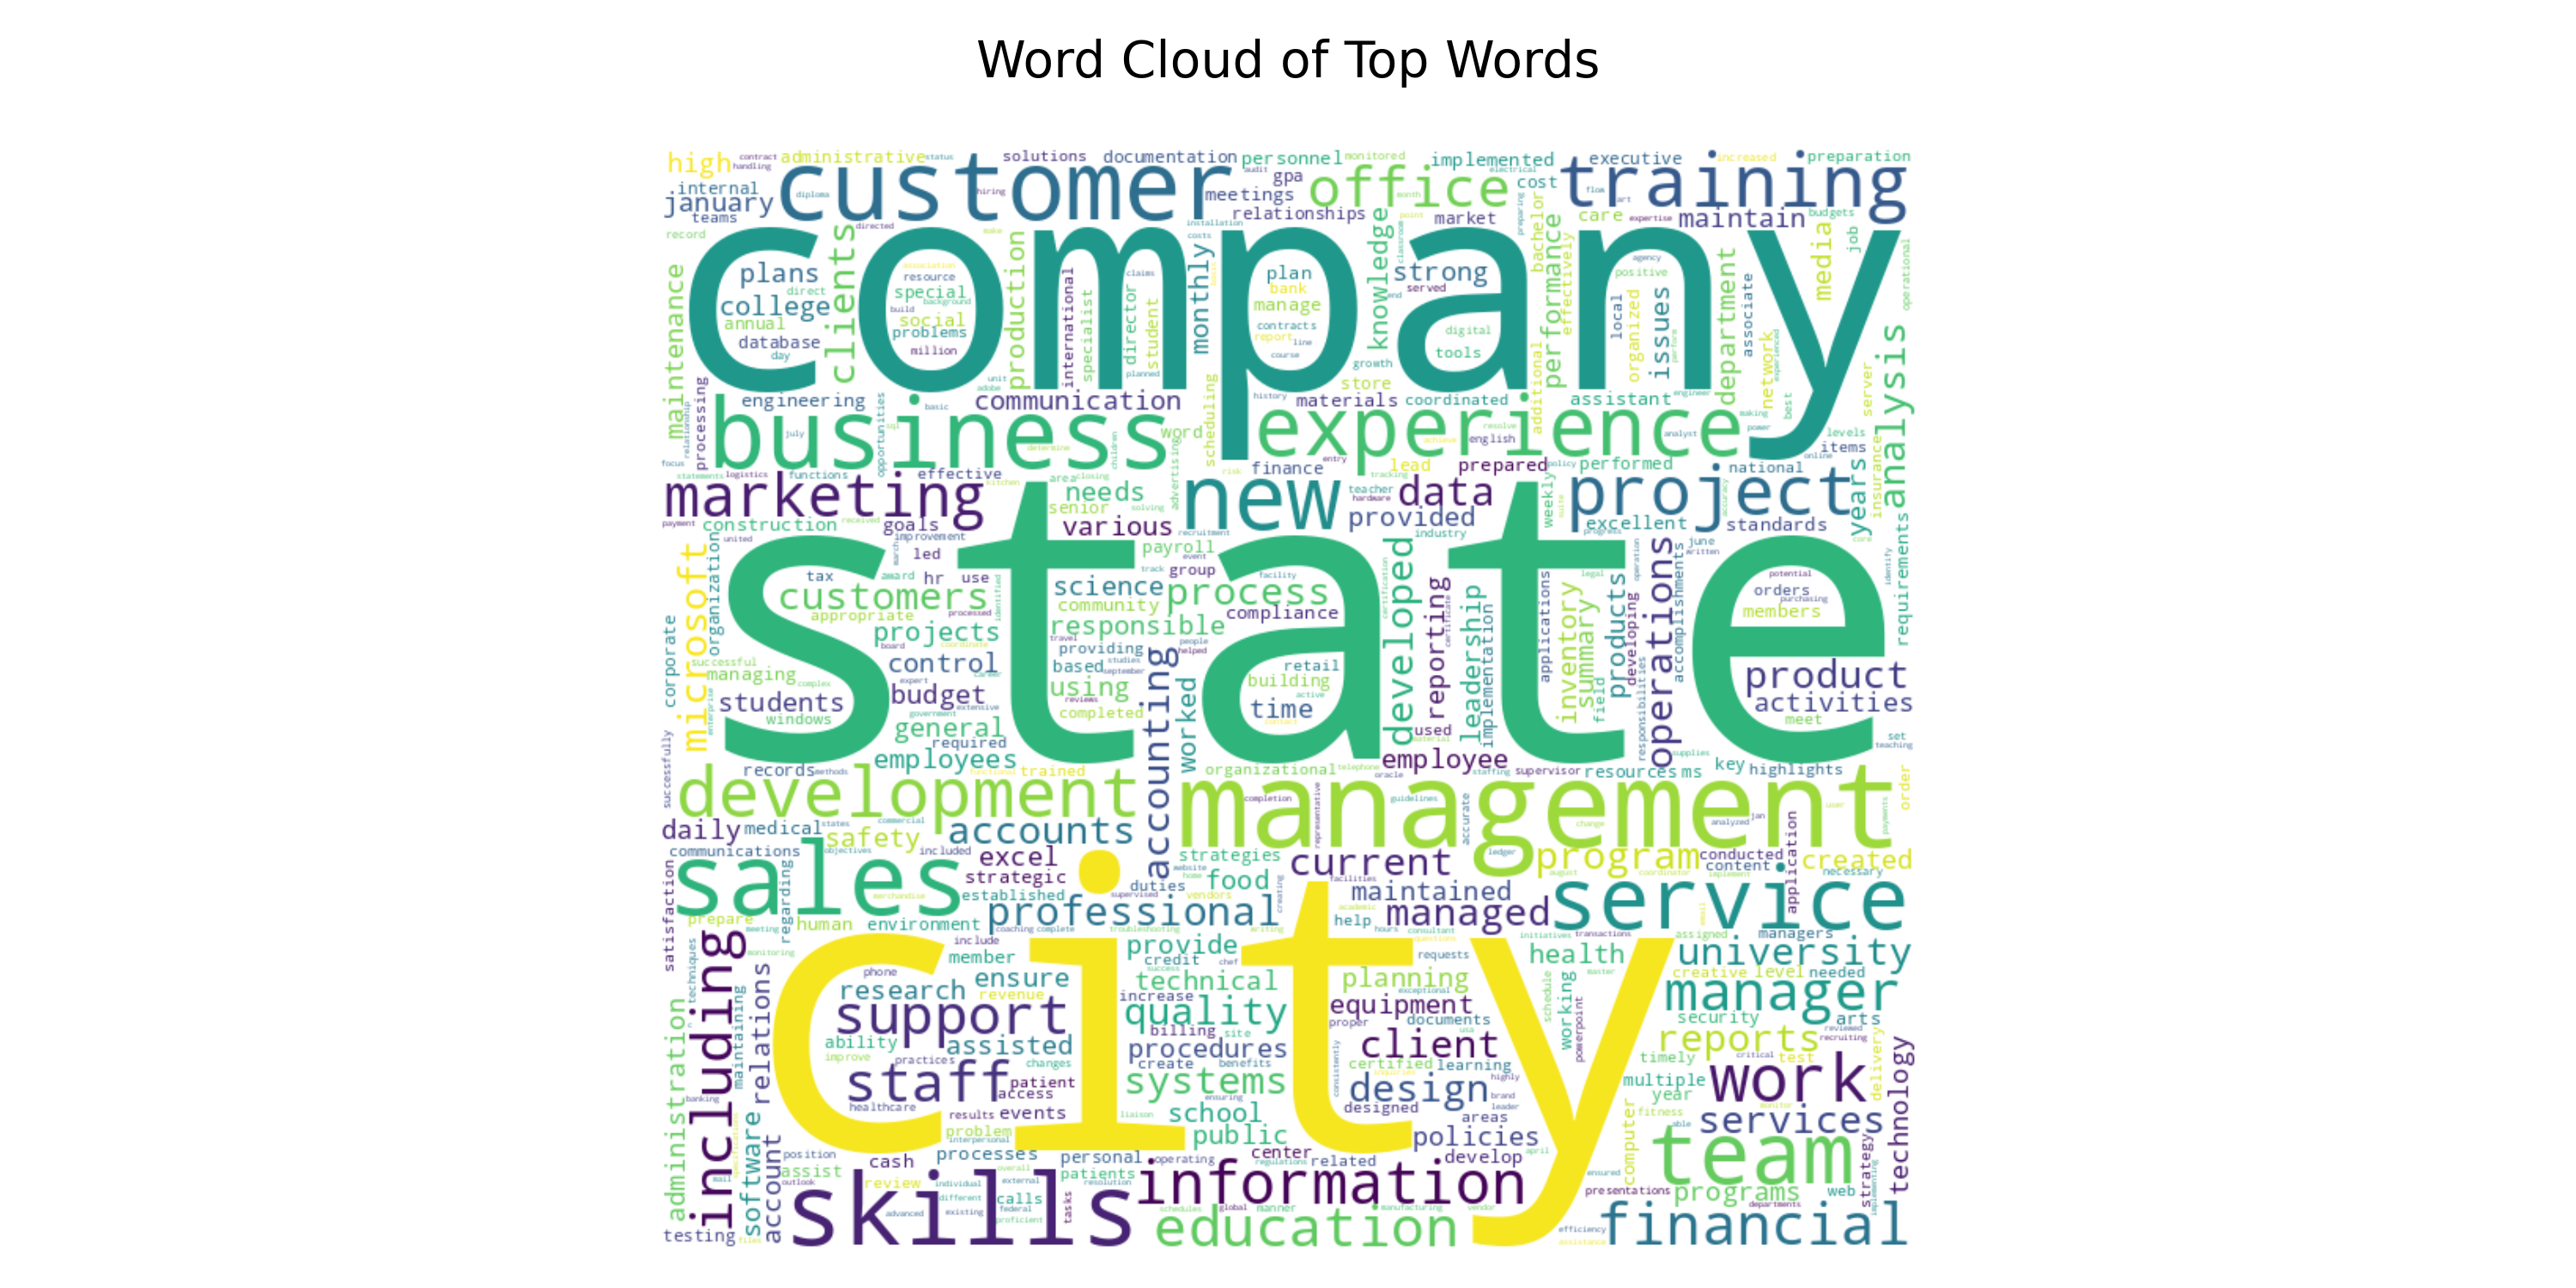
\includegraphics[width=0.8\textwidth]{../src/data/wordcloud/wordcloud_overall.png}
    \caption{WordCloud globale dei termini più frequenti nei curriculum.}
\end{figure}

\section{Struttura del Progetto e Moduli Ausiliari}
Per mantenere il codice pulito e modulare, abbiamo organizzato le funzioni di utilità in un pacchetto dedicato denominato \texttt{tools}.

\subsection{Modulo Utils (\texttt{utils.py})}
In questo modulo abbiamo implementato le logiche di manipolazione del testo:
\begin{itemize}
    \item \texttt{preprocess\_text}: gestisce la pulizia avanzata, inclusa la rimozione delle intestazioni in maiuscolo.
    \item \texttt{top\_in\_series}: calcola le frequenze dei termini escludendo le stop words.
\end{itemize}

\subsection{Modulo Plotting (\texttt{plotting.py})}
Questo modulo incapsula la logica di visualizzazione, in particolare la generazione delle WordCloud, permettendoci di riutilizzare le stesse impostazioni grafiche in diversi notebook.

\section{Metodologia}
Per l'implementazione dei modelli e la gestione dei dati è stato utilizzato il framework \textbf{Scikit-learn} \cite{sklearn}.

\subsection{Suddivisione dei Dati}
Abbiamo suddiviso il dataset in tre partizioni per garantire una valutazione robusta del modello:
\begin{itemize}
    \item \textbf{Training Set (70\%)}: Utilizzato per l'addestramento dei parametri del modello.
    \item \textbf{Validation Set (15\%)}: Riservato per l'ottimizzazione degli iperparametri (Hyperparameter Tuning). In questa fase di \textit{baseline}, il modello è stato valutato con parametri di default, ma questo set rimane essenziale per futuri esperimenti di selezione del modello senza \"contaminare\" il test set.
    \item \textbf{Test Set (15\%)}: Utilizzato esclusivamente per la valutazione finale delle performance su dati mai visti.
\end{itemize}

\textit{Nota metodologica:} In uno scenario di produzione reale, l'uso di una singola suddivisione Train/Val/Test può essere soggetto a varianza statistica, specialmente con dataset di dimensioni ridotte. Una stima più robusta delle performance richiederebbe l'applicazione della **K-Fold Cross-Validation**, che tuttavia non è stata implementata in questa iterazione per mantenere la pipeline computazionalmente leggera. Inoltre, la scelta di utilizzare l'accuracy come metrica globale è parzialmente limitata dallo sbilanciamento delle classi; per questo motivo, nella sezione Risultati, viene data priorità all'analisi di Precision, Recall e F1-Score per classe.

La suddivisione è stata effettuata in modo stratificato rispetto alla variabile target \texttt{Category} per mantenere le proporzioni delle classi.

\subsection{Feature Extraction: TF-IDF}
Per trasformare il testo in vettori numerici utilizzabili dagli algoritmi di Machine Learning, abbiamo scelto la tecnica \textbf{TF-IDF (Term Frequency - Inverse Document Frequency)} \cite{tfidf}.

\textbf{Motivazione della scelta e confronto:}
Abbiamo preferito TF-IDF rispetto al semplice modello **Bag of Words (BoW)** poiché quest'ultimo considera esclusivamente la frequenza dei termini, rischiando di assegnare un peso eccessivo a parole molto comuni ma poco informative.
Per quanto riguarda tecniche più avanzate basate su **Word Embedding** (come Word2Vec o modelli Transformer tipo BERT), sebbene l'utilizzo di modelli pre-addestrati (Transfer Learning) rappresenti oggi lo stato dell'arte per catturare relazioni semantiche, abbiamo scelto in questa fase di utilizzare TF-IDF per stabilire una **baseline solida**. Questo approccio garantisce:
\begin{itemize}
    \item \textbf{Interpretabilità}: È possibile risalire esattamente a quali parole determinano la classificazione.
    \item \textbf{Efficienza}: Richiede risorse computazionali minime (CPU) rispetto ai modelli Transformer (GPU).
\end{itemize}
L'accuratezza ottenuta (vedi sez. Risultati) evidenzia tuttavia i limiti di questo approccio nel catturare sinonimi e contesto, suggerendo che l'integrazione futura di Embeddings potrebbe migliorare significativamente le performance.

Configurazione utilizzata:
\begin{itemize}
    \item \textbf{max\_features}: 5000 (per limitare la dimensionalità).
    \item \textbf{ngram\_range}: (1, 2) (per considerare sia parole singole che bigrammi).
    \item \textbf{stop\_words}: 'english' (per rimuovere parole comuni prive di significato semantico).
\end{itemize}

\textit{Nota metodologica e Critica:} La configurazione attuale presenta due limitazioni teoriche importanti:
\begin{enumerate}
    \item \textbf{Stop Words Generiche:} L'uso della lista standard 'english' non filtra il rumore specifico del dominio. Termini onnipresenti nei CV come "experience", "skills", "worked", "team" o "responsible" non portano informazione discriminante ma non vengono rimossi, "inquinando" lo spazio vettoriale. Una lista di \textit{custom stop words} sarebbe stata preferibile.
    \item \textbf{Taglio Dimensionale (max\_features=5000):} Sebbene riduca il costo computazionale, limitare arbitrariamente il vocabolario è teoricamente sub-ottimale per le SVM, che sono note per gestire eccellentemente spazi ad altissima dimensionalità (anche >100.000 feature). Questo taglio rischia di eliminare la "coda lunga" di termini tecnici rari (es. uno specifico software di nicchia) che spesso sono i predittori più forti per categorie specifiche.
\end{enumerate}
Inoltre, l'attuale feature engineering si basa esclusivamente su n-grammi di parole. Una rappresentazione più ricca potrebbe includere metadati strutturali del CV (es. lunghezza del testo, presenza di sezioni standard) o feature linguistiche.

\begin{lstlisting}[language=Python, caption=Configurazione TF-IDF]
vectorizer = TfidfVectorizer(stop_words='english', max_features=5000, ngram_range=(1, 2))
X_train_vec = vectorizer.fit_transform(X_train)
\end{lstlisting}

\textit{Nota metodologica (Prevenzione Data Leakage):} È fondamentale sottolineare che il metodo \texttt{fit\_transform} è stato applicato \textbf{solo} al Training Set. Per il Validation e il Test Set (e in fase di inferenza), si utilizza esclusivamente il metodo \texttt{transform}. Questo garantisce che il vocabolario e i pesi IDF siano appresi solo dai dati di addestramento, evitando che informazioni del test set "trapelino" nel modello (Data Leakage), il che porterebbe a stime delle performance eccessivamente ottimistiche e non realistiche.

\subsection{Modello di Classificazione: Linear SVC}
Come classificatore, abbiamo optato per una \textbf{Linear Support Vector Machine (LinearSVC)} \cite{svm}.

\textbf{Motivazione della scelta e confronto:}
Le SVM lineari sono note per la loro efficacia su spazi di feature ad alta dimensionalità e sparsi, tipici delle rappresentazioni testuali come TF-IDF.
Rispetto ad altre alternative comuni:
\begin{itemize}
    \item \textbf{Naive Bayes (MultinomialNB)}: Costituisce una baseline standard per il testo grazie alla sua velocità, ma le SVM tendono spesso a superarlo in accuratezza poiché cercano il margine di separazione ottimale tra le classi, gestendo meglio le interazioni tra termini.
    \item \textbf{Modelli basati su Alberi (Random Forest / XGBoost)}: Sebbene molto potenti su dati tabellari densi, possono risultare computazionalmente inefficienti su vettori sparsi ad altissima dimensionalità (come il vocabolario TF-IDF di 5000 feature) senza un'adeguata riduzione dimensionale (es. LSA/SVD).
    \item \textbf{Deep Learning}: L'utilizzo di Reti Neurali Feed-Forward semplici su TF-IDF raramente supera le SVM lineari. Il vero salto di qualità richiederebbe architetture ricorrenti (RNN) o Transformer (BERT) che lavorano su sequenze e non su "sacchi di parole", rappresentando il naturale sviluppo futuro di questo progetto.
\end{itemize}

\begin{lstlisting}[language=Python, caption=Addestramento del modello LinearSVC]
from sklearn.svm import LinearSVC

model = LinearSVC(random_state=42, dual='auto')
model.fit(X_train_vec, y_train)
\end{lstlisting}

\textit{Nota Critica (Gestione dello Sbilanciamento):} Si noti che il modello è stato istanziato con i pesi di default. Dato il forte sbilanciamento delle classi evidenziato in fase di analisi (es. classi con rapporto 1:6), sarebbe stato opportuno utilizzare il parametro \texttt{class\_weight='balanced'}. Questa modifica avrebbe penalizzato maggiormente gli errori sulle classi minoritarie, potenzialmente migliorando la Recall per categorie come \textit{BPO} o \textit{AUTOMOBILE}, a discapito forse di una leggera riduzione della precisione globale.

\section{Risultati}

\subsection{Performance sul Test Set}
Il modello ha raggiunto un\'accuratezza complessiva (Accuracy) di circa il \textbf{52\%} sul Test Set.
Di seguito riportiamo un estratto delle metriche di classificazione per alcune categorie:

\begin{table}[H]
\centering
\begin{tabular}{lccc}
\toprule
\textbf{Categoria} & \textbf{Precision} & \textbf{Recall} & \textbf{F1-Score} \\
\midrule
CHEF & 0.84 & 0.94 & 0.89 \\
DIGITAL-MEDIA & 1.00 & 0.71 & 0.83 \\
ENGINEERING & 0.75 & 0.67 & 0.71 \\
TEACHER & 0.55 & 0.80 & 0.65 \\
HR & 0.52 & 0.76 & 0.62 \\
FINANCE & 0.43 & 0.33 & 0.38 \\
\bottomrule
\end{tabular}
\caption{Metriche principali per un sottoinsieme rappresentativo di categorie.}
\end{table}

Come si evince, alcune categorie come \textit{CHEF} e \textit{DIGITAL-MEDIA} sono classificate con alta precisione, grazie probabilmente a un vocabolario tecnico molto specifico (es. nomi di ingredienti o software). Al contrario, categorie come \textit{FINANCE} o \textit{HR} mostrano performance inferiori, soffrendo della sovrapposizione terminologica con altre aree aziendali (es. \textit{ACCOUNTANT}, \textit{BUSINESS-DEVELOPMENT}).

\subsection{Matrice di Confusione e Analisi degli Errori}
Abbiamo analizzato la matrice di confusione per comprendere le cause dell'accuratezza (52\%), che risulta inferiore allo stato dell'arte per questo tipo di task (generalmente >70\%).
L'analisi degli errori suggerisce che il modello TF-IDF fatica a distinguere categorie con forte \textbf{sovrapposizione semantica} (Semantic Overlap). Ad esempio, i termini presenti nei CV di \textit{SALES} (vendite) e \textit{BUSINESS-DEVELOPMENT} sono spesso identici (es. "client", "revenue", "target").
Il modello lineare, basandosi sulla presenza esatta delle parole (keyword matching) e non sul loro significato contestuale, non riesce a discriminare queste sfumature. Questo conferma l'ipotesi che l'introduzione di \textbf{Word Embeddings} (che mappano parole diverse ma simili nello stesso spazio vettoriale) sia l'intervento correttivo prioritario.

\begin{figure}[H]
    \centering
    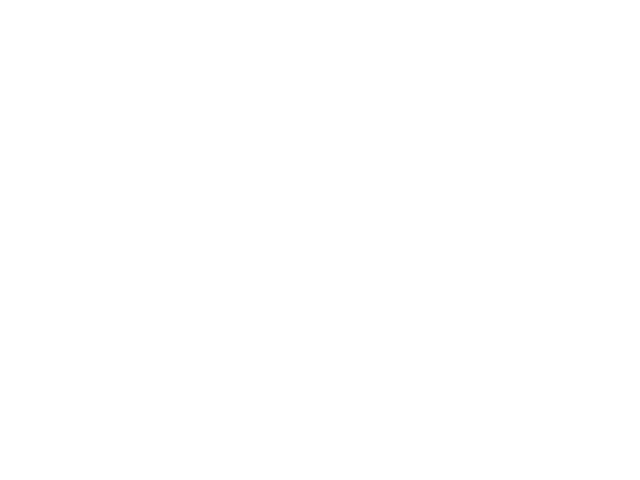
\includegraphics[width=0.8\textwidth]{../src/data/confusion_matrix.png}
    \caption{Matrice di Confusione generata dallo script di training.}
\end{figure}

\section{Inferenza e Messa in Produzione}
Un aspetto cruciale della pipeline è la capacità di effettuare previsioni su nuovi dati. Abbiamo implementato una funzione di inferenza che accetta una stringa grezza (il testo di un nuovo CV), applica la stessa catena di preprocessing e vettorizzazione (utilizzando il vocabolario appreso durante il training) e restituisce la categoria predetta.

\begin{lstlisting}[language=Python, caption=Esempio di Inferenza su un nuovo CV]
def predict_category(resume_text, model, vectorizer):
    # 1. Cleaning con la stessa logica del training
    clean_resume = clean_text(resume_text)
    # 2. Trasformazione (SOLO transform, mai fit!)
    vec = vectorizer.transform([clean_resume])
    # 3. Predizione
    return model.predict(vec)[0]
\end{lstlisting}

Questa struttura garantisce che il sistema sia pronto per essere integrato in un'applicazione web o una REST API.

\textit{Critica Operativa (Mancanza di Score di Confidenza):} Un limite dell'attuale implementazione \texttt{LinearSVC} è che restituisce solo la classe predetta senza una probabilità associata. In un contesto di produzione, è fondamentale avere un **confidence score** per gestire i casi incerti (es. richiedere revisione umana se la confidenza è < 70\%). Per il futuro, si suggerisce di calibrare il modello (es. con \texttt{CalibratedClassifierCV}) o valutare modelli probabilistici nativi come la Logistic Regression.

\section{Conclusioni e Sviluppi Futuri}
In questo progetto abbiamo sviluppato con successo una pipeline end-to-end per la classificazione di curriculum. L\'utilizzo di TF-IDF combinato con LinearSVC ha fornito una baseline solida, evidenziando sia i punti di forza (velocità, interpretabilità) che i limiti (mancanza di contesto semantico) degli approcci classici.
Sviluppi futuri potrebbero includere:
\begin{itemize}
    \item Utilizzo di embedding pre-addestrati (es. Word2Vec, GloVe o BERT) per catturare meglio il contesto semantico.
    \item Bilanciamento delle classi tramite tecniche di oversampling (es. SMOTE) per le categorie meno rappresentate.
    \item Ottimizzazione degli iperparametri del modello SVM.
\end{itemize}

\begin{thebibliography}{9}
\bibitem{tfidf}
Salton, G., \& McGill, M. J. (1983). \textit{Introduction to modern information retrieval}. McGraw-Hill.

\bibitem{sklearn}
Pedregosa, F., et al. (2011). Scikit-learn: Machine Learning in Python. \textit{Journal of Machine Learning Research}, 12, 2825-2830.

\bibitem{svm}
Joachims, T. (1998). Text categorization with Support Vector Machines: Learning with many relevant features. \textit{European conference on machine learning}.
\end{thebibliography}
\end{document}
